
%%%
%%% CHAPTER
%%%
\chapter{Thermodynamics: Introduction and Principles}\label{Chapter:Introduction}


   \begin{LearningObjectivesBlock}{Learning Objectives}
      Upon completion of this chapter, you will
        \begin{enumerate}
           \item be able to identify the main elements in a thermodynamic system;
           \item understand the concept of thermodynamic equilibrium;
           \item be able to state the zeroth law of thermodynamics.
        \end{enumerate}
\medskip
     Recommended reading: Chapter 2 of \citet{Atkins_Book,Devoe_Book,Borgnakke_Book}.
   \end{LearningObjectivesBlock}

%%%% ETOC
\etocsetnexttocdepth{subsection}
\localtableofcontents

%%%
%%% SECTION
%%%
   \section{Introduction}\label{Chapter:Introduction:Section:Introduction}

   The word `{\it thermodynamics}' stems from Greek roots, {\it therme}: heat and {\it dynamis}: power -- `movement of heat', and was used by the first time by Lord Kelvin \citep{Thomson_1849}. Thermodynamics studies global properties of the matter and the process (\eg thermal, chemical, mechanical, nuclear etc) in which these properties may be altered. In other words, the quantification of the inter-relation between energy and the change of properties of any physical system.

   For most practical applications, thermodynamics deals with interactions between thermal (\ie heat and temperature), mechanical (\ie work) and/or chemical (\ie chemical potential) energies. \citet{Borgnakke_Book} defined thermodynamics as the `the science that deals with heat and work and those properties of matter that relate to heat and work.'

   \medskip
   
   The study of thermodynamics may be divided into two main areas, {\it classical} and {\it statistical} thermodynamics. The latter investigates the macroscopic properties of systems comprising of a large number of subsystems (\ie particles or atoms). Properties of such systems are controlled by the motion of each set (or assembly) of particles, which can be determined by applying probabilistic theories and methods to laws of motion.

   {\it Classical thermodynamics} studies macroscopic changes of properties, \ie it is assumed that matter is formed by large quantity of particle assemblies that have properties representing the interactions between these assemblies. The extent of such changes due to transfer of energy to or from the system is described by fundamental equations of thermodynamics which are derived from observations known as `{\it Laws of Thermodynamics}'. These laws are postulates that describe the nature of interactions of systems and energy.

   {\bf This document will focus only on the study of fundamentals of \underline{classical thermodynamics} and its application on environmental and industrial problems. }

%%%
%%% SECTION
%%%
   \section{Main Elements of Thermodynamics Analysis}\label{Chapter:Introduction:Section:ThermodAnalysis}

   The first stage in the analysis of any thermodynamic problem is to identify the domain in which all energy and/or forces are transferred to or from.
% Figure
   \begin{figure}[h]
     \begin{center}
       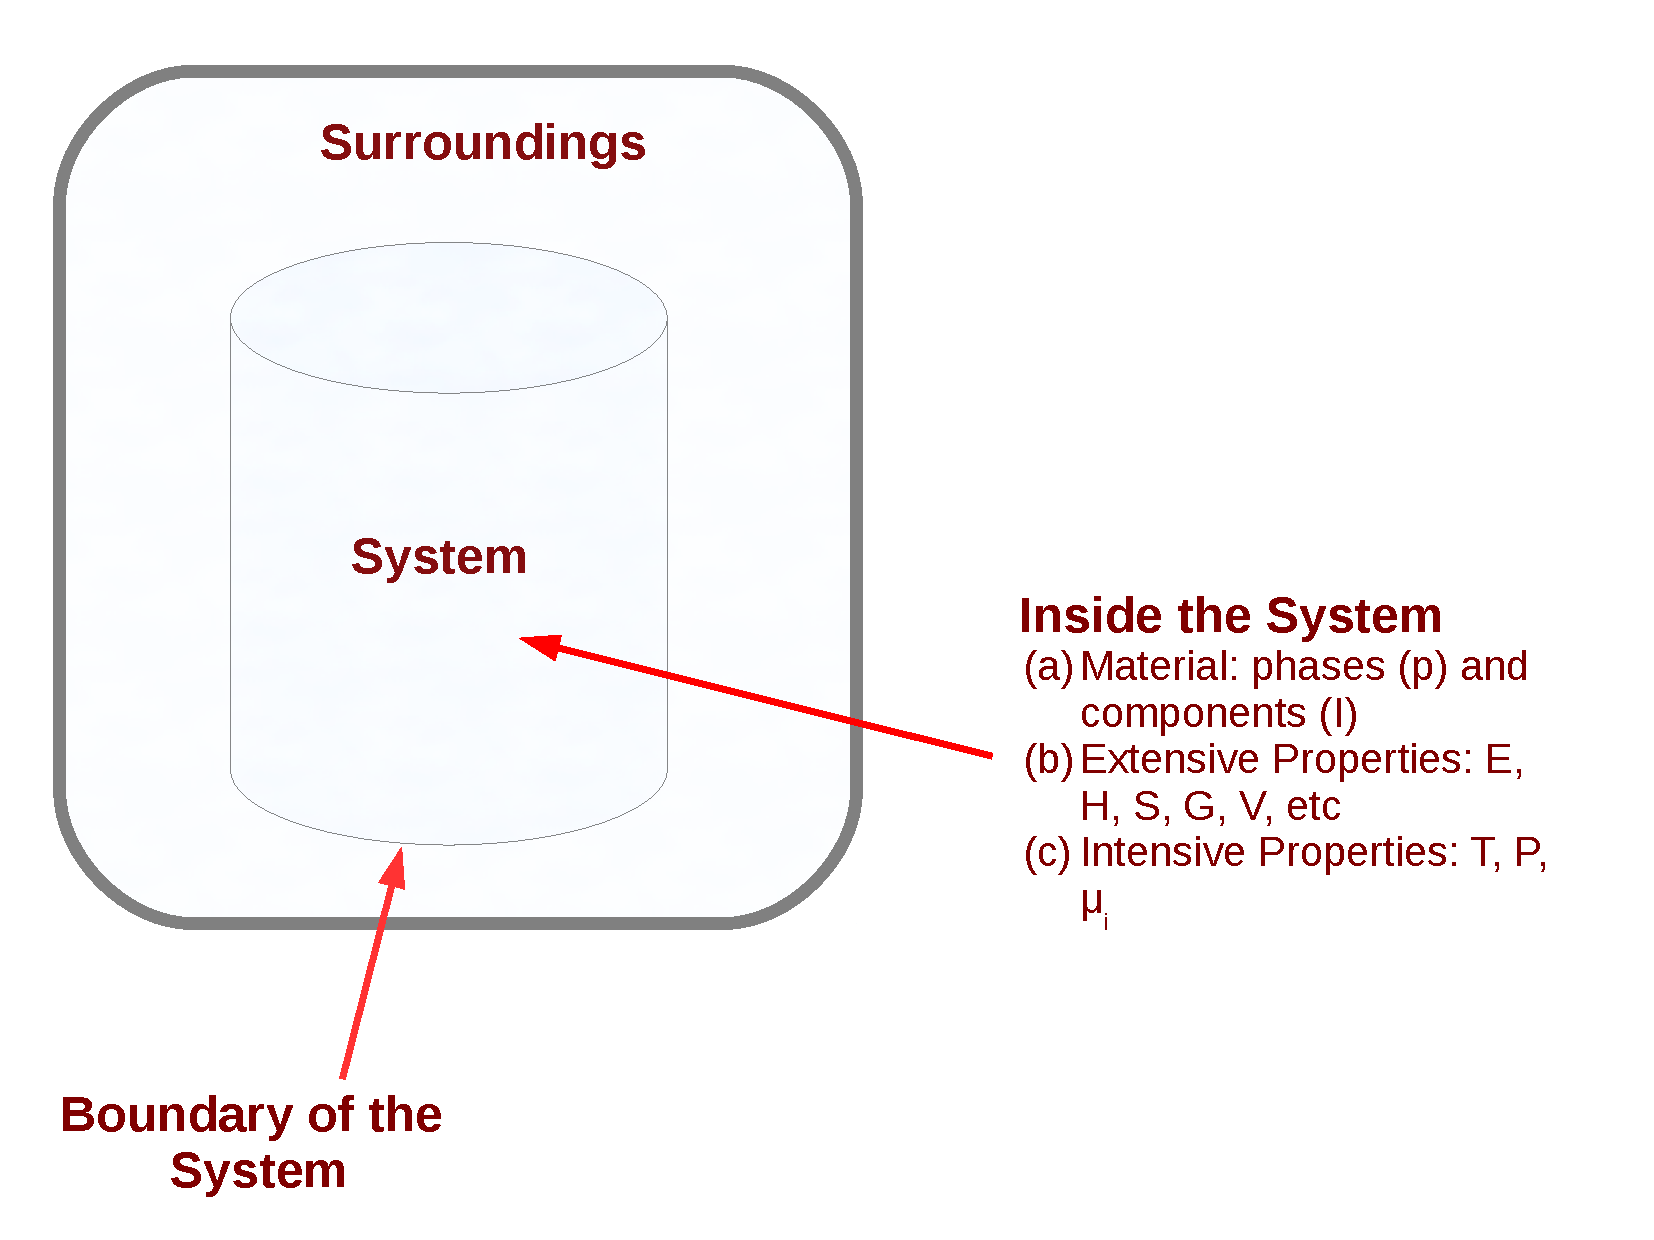
\includegraphics[width=8cm, height=8cm]{./../Pics/Fig_SystemDefinition}
       \caption{Elements of a thermodynamic problem: system and surroundings separated by well-defined borders.}\label{Chapter:Introduction:Fig:Domain}
     \end{center}
   \end{figure}
   
   
%%% Subsection
   \subsection{System, Surroundings and Boundaries}\label{Chapter:Introduction:Section:Introduction:SystemSurroundingsBoundaries}\index{System}\index{System!Boundaries}\index{System!Surroundings}
   In practice, any thermodynamic analysis starts by defining the domain of interest, which can be a volume in space or quantity of matter (Fig.~\ref{Chapter:Introduction:Fig:Domain}). This domain is called {\it system}, \ie any 3-D region of physical space with prescribed mass; the remaining of the domain is called {\it surroundings} (or {\it neighbourhood}) which is limited by {\it boundaries}. The {\it boundary} is a surface that encloses the {\it system} and separates it from the {\it surroundings}. For example, in Fig.~\ref{Chapter:Introduction:Fig:Domain2}, liquid nitrogen is contained in a cylinder with prescribed wall thickness. In this case, the interior of the vessel with N$_{2}$ is the {\it system}, whereas the cylinder wall is the border of the system. 
% Figure
   \begin{wrapfigure}{I}{0.5\columnwidth}
        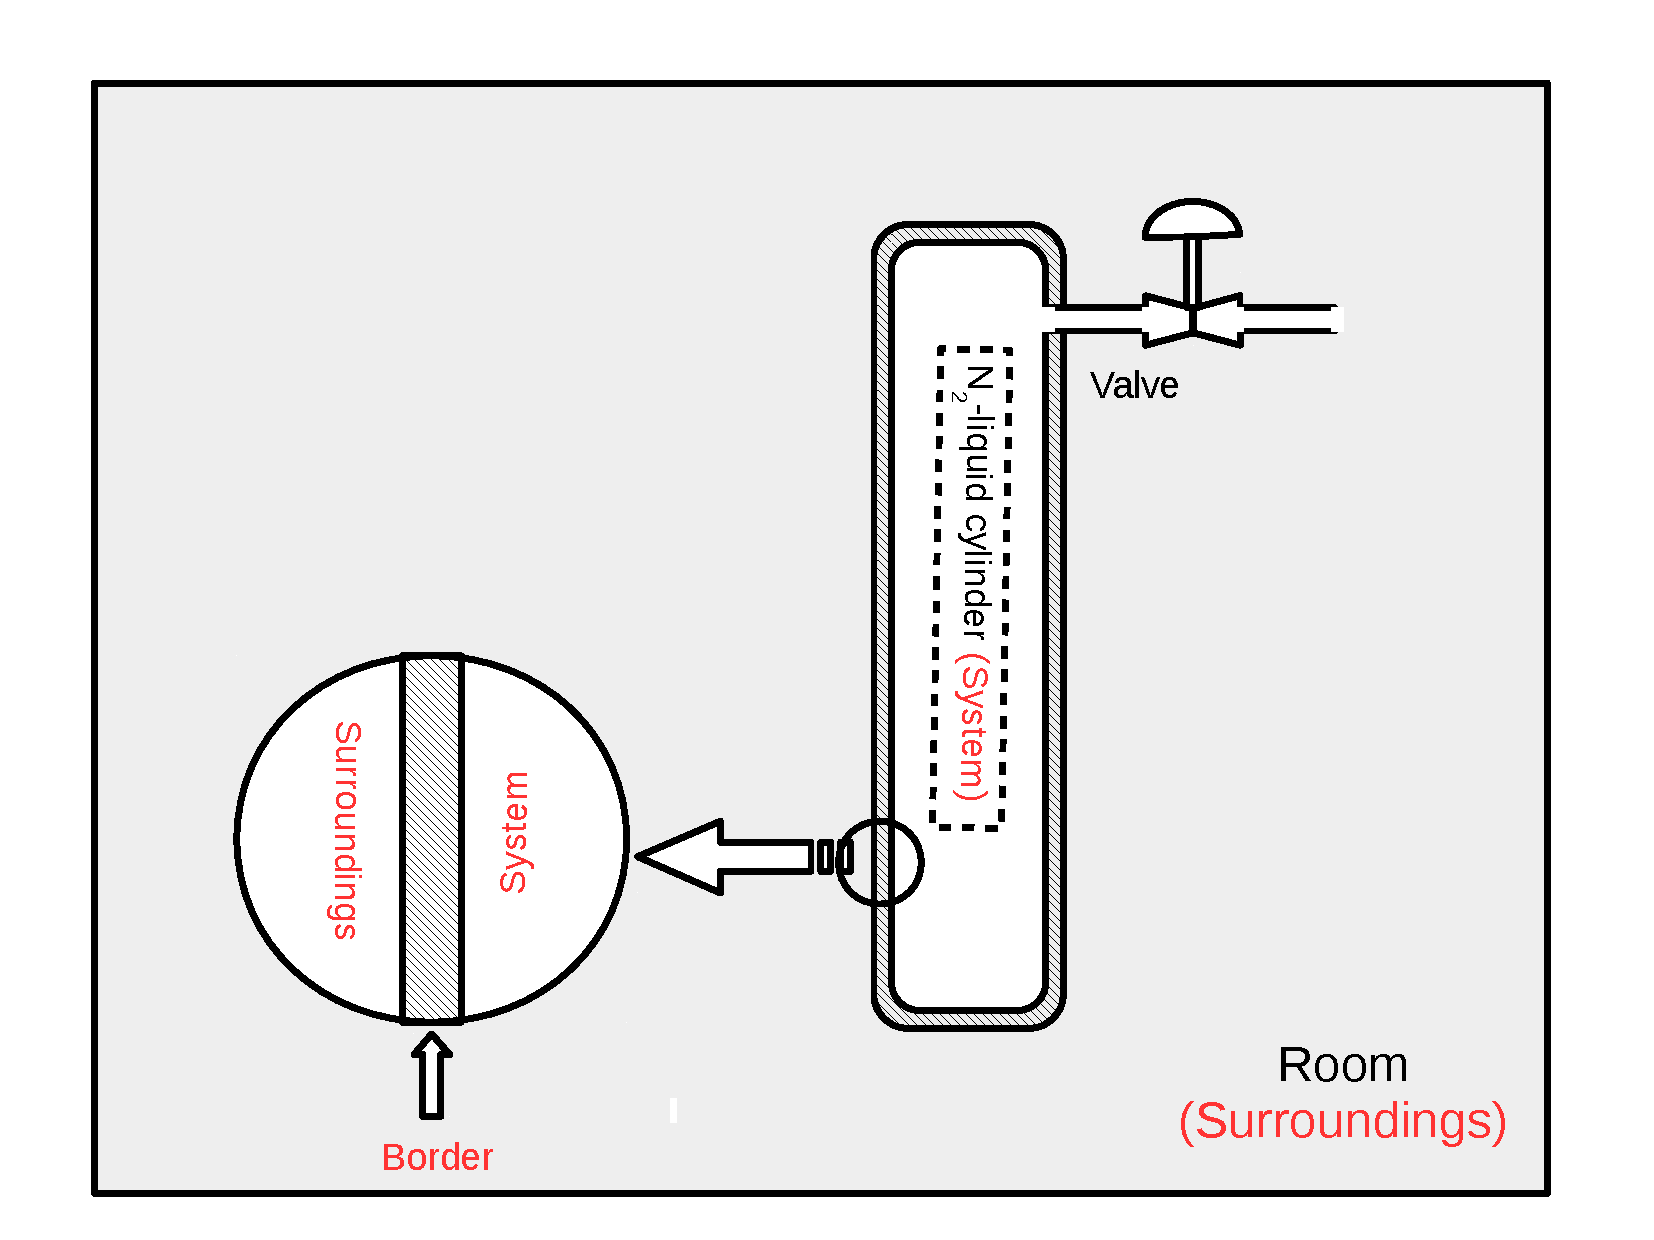
\includegraphics[width=0.4\columnwidth,clip]{./../Pics/Fig_SystemDefinition2}
        \caption{Example of a well-defined thermodynamic problem: cylinder stored in a room. Pressurised liquid N$_{2}$ contained in a cylinder is the system, whereas the remaining of the room are the surroundings. Cylinder's wall is the border of the system.}\label{Chapter:Introduction:Fig:Domain2}
   \end{wrapfigure}

   For convenience, sometimes we may want to divide the {\it system} into multiple {\it sub-systems} and analyse them individually, or to combine several small {\it systems} into larger {\it super-systems}. The choice depends on the conditions of the domain of interest and how mass and energy flow across the {\it sub-systems}. For example, in Fig.~\ref{Chapter:Introduction:Fig:Domain2}, if the valve is opened to the room (at atmospheric pressure) $N_{2}$ would be vaporised ({\it phase change}) and occupy the whole room. In such scenario, the room and the cylinder become the {\it system} bounded by the room's walls; the area outside the room is now the surroundings. Multiple different configurations can be drawn from this rather simple cylinder-room set.

%%% Table
   \begin{table}[h]
     \begin{center}
      \begin{tabular}{|c|c|c|}
         \hline
                      & {\bf Mass} & {\bf Energy} \\
                      & {\bf Exchange} & {\bf Exchange} \\
         \hline
         {\bf Open}   & {\it yes}  & {\it yes}    \\
         {\bf Closed} & {\it no}   & {\it yes}    \\
         {\bf Isolated}&{\it no}   & {\it no}     \\
         \hline 
      \end{tabular}  
        \caption{System and control volumes: energy and mass transfer.}\label{Chapter:Introduction:Table:System}
     \end{center}
   \end{table}
   
   If mass and energy are allowed to flow across the {\it boundaries}, we say that the {\it system} is {\bf open}, otherwise if only the energy is allowed to flow (\ie be transferred) across the {\it boundaries}, the {\it system} is assumed to be {\bf closed}. If both energy and mass can not be transferred across the {\it boundaries} the system is assumed {\bf isolated}, in such case, where there is no energy flow, the boundary is called {\bf adiabatic} (Table~\ref{Chapter:Introduction:Table:System}).\index{System!Open}\index{System!Closed}\index{System!Isolated}\index{System!Adiabatic}\index{Adiabatic}

% Figure
   \begin{figure}[h]
     \begin{center}
        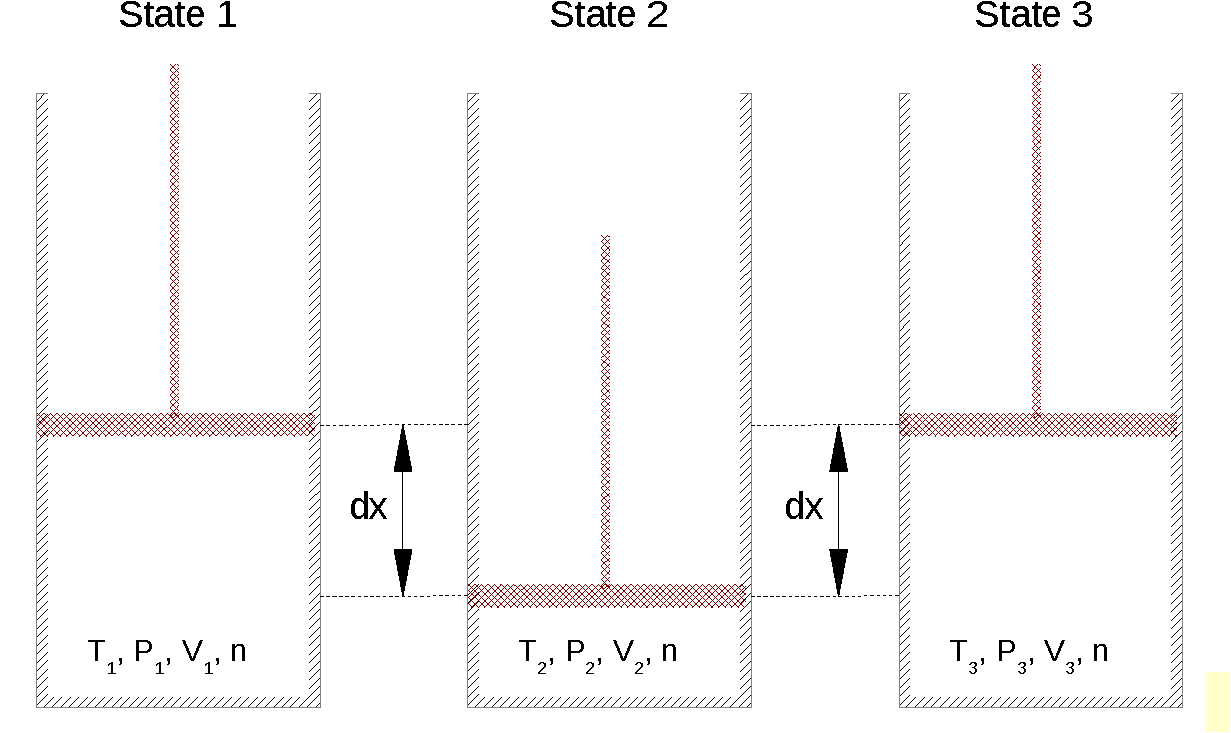
\includegraphics[width=0.7\columnwidth,clip]{./../Pics/Fig_SystemDefinition3}
        \caption{Cylinder-piston system with extensive/intensive properties.}\label{Chapter:Introduction:Fig:Domain3}
     \end{center}
   \end{figure}

   In the example depicted in Fig.~\ref{Chapter:Introduction:Fig:Domain2}, assuming an ordinary industrial liquid N$_{2}$ (at subzero temperature) cylinder, if the valve is closed, then there is no fluid flow from the cylinder to the room, but heat is flowing from the environment to the cylinder cavity. Such system is said to be {\bf closed}.
   
\medskip
% Example
\begin{MyExample}{\begin{center}{\bf Example}\end{center}}
\begin{example}\label{Chapter:Introduction:Example1}
  \citep{Reisel_Book} For the following systems, determine whether the system described is best modelled as an isolated, closed or open system:
  \begin{enumerate}[a)]
     \item steam flowing through a turbine\;\;$\rightarrow$\;\; {\it Open.}
     \item an incandescent light bulb\;\;$\rightarrow$\;\; {\it Closed.}
     \item an inflated tire\;\;$\rightarrow$\;\; {\it Isolated if the tire is at rest, but closed if it is in movement.}
     \item a rock formation 200 m below the surface of the earth\;\;$\rightarrow$\;\; {\it Open.}
     \item a tea kettle containing boiling water\;\;$\rightarrow$\;\; {\it Open as water steam can still leave the system.}
     \item a human body\;\;$\rightarrow$\;\;{\it Depending on the circumstances, a human body can be either open (\eg during meals, physical exercises etc) or closed.}
     \item an engine's radiator\;\;$\rightarrow$\;\; {\it Closed}.
  \end{enumerate}
\end{example}
\end{MyExample}

%%% Subsection
   \subsection{Properties and State of Substances}\label{Chapter:Introduction:Section:Introduction:ExtensiveIntensiveProperties}\index{Extensive Properties}\index{Intensive Properties}\index{System!Extensive Properties}\index{System!Intensive Properties}
   The {\it material} in a system is composed of phases (e.g., solid, liquid, gas) with distinct physical and chemical properties, thus with explicit {\it boundaries} (\ie interfaces) between phases. {\it State} is the condition of the system at an instant of time and described by its properties.  From this definition of state, any property has a single value at each state. A quantitative property of a system (\eg temperature and pressure) describes macroscopic characteristics, which may vary with time (\ie time-dependent property). Two states of the matter are equivalent if they have the same properties, \eg in a cylinder-piston system (Fig.~\ref{Chapter:Introduction:Fig:Domain3}) containing {\it n} moles of pure gas, if {\it state 1} is defined by temperature $T_{1}$, pressure $P_{1}$ and volume $V_{1}$, and {\it state 3} is defined by temperature $T_{3}$, pressure $P_{3}$ and volume $V_{3}$, state 1 is {\it equivalent} to state 3 {\it if and only if} $T_{1} = T_{3}$ and $P_{1} = P_{2}$. 
\medskip

   Thermodynamic properties may be classified as either {\bf extensive} or {\bf intensive}. An extensive property is a property that depends on the mass (or extent) of the substance (\ie size) in the system. Examples of extensive properties are total mass, total volume, total internal energy etc. An intensive property is a property that is independent of the mass of the substance, examples are temperature and pressure.
% Figure
   \begin{wrapfigure}{R}{0.5\columnwidth}
        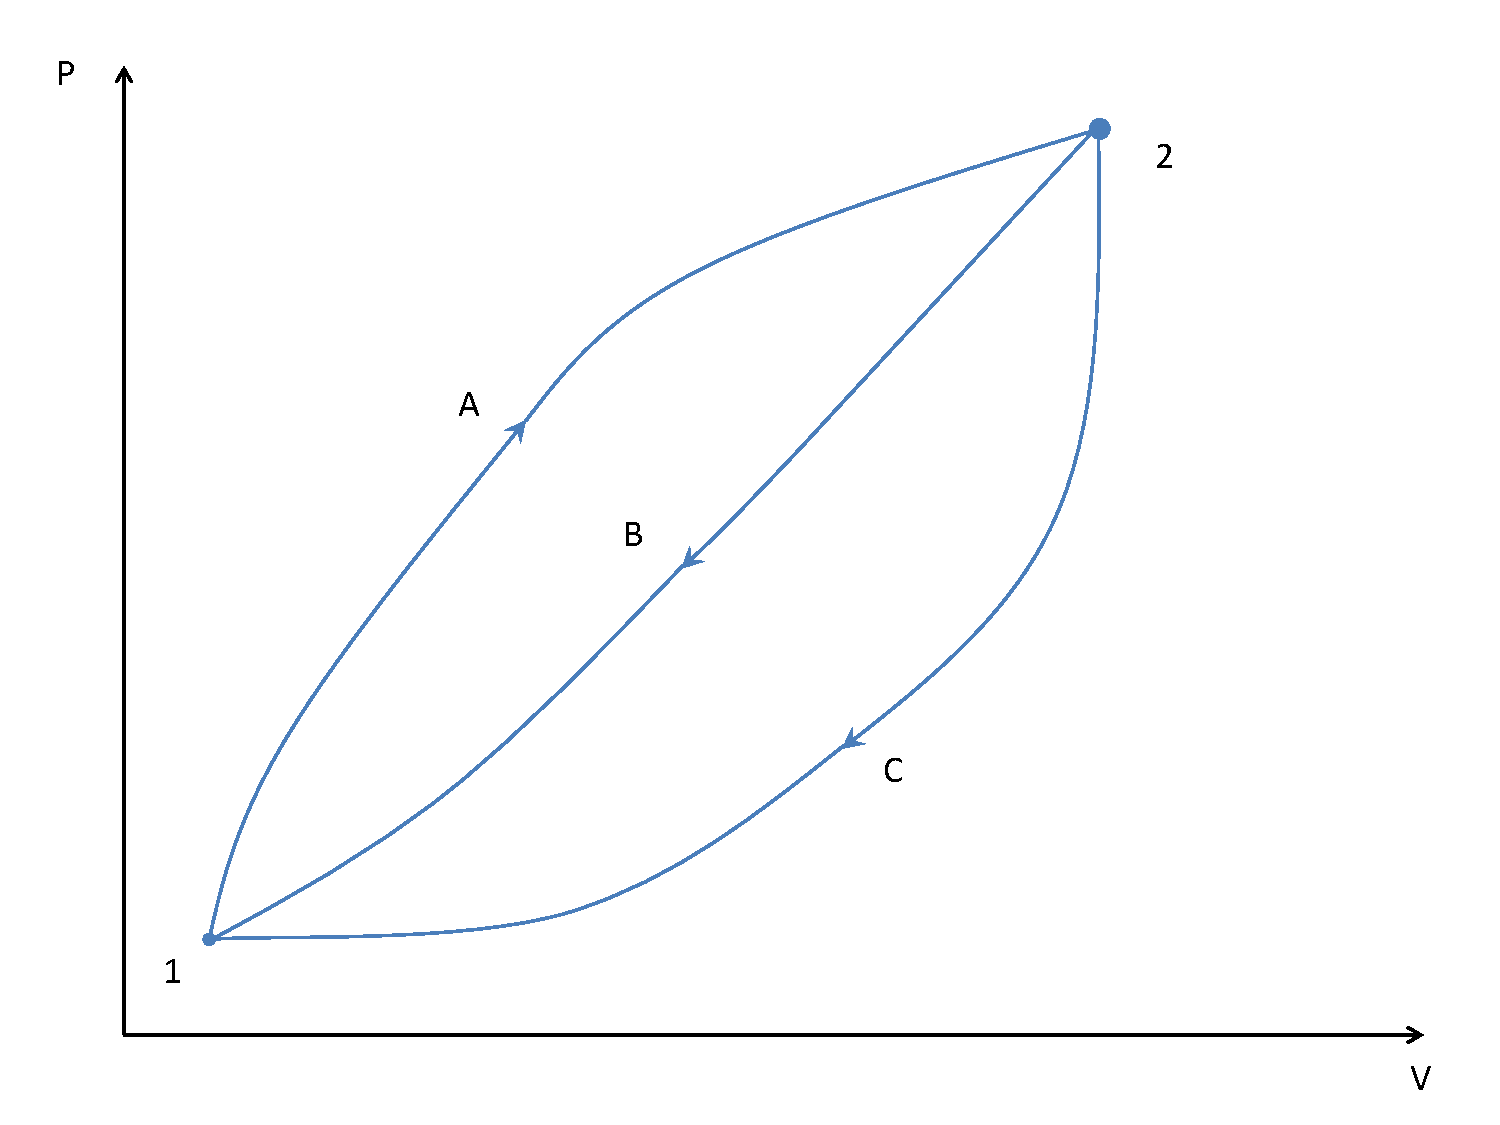
\includegraphics[width=0.4\columnwidth,clip]{./../Pics/first_law_process}
        \caption{Schematic representation of cycles.}\label{Chapter:Introduction:Fig:CyclesSchematic}
   \end{wrapfigure}

   Thus, for example, if a system is cut in half, its intensive properties remain unchanged, while extensive properties are cut in half. The ratio of an extensive property to the mass (\ie property per unit mass) is called {\bf specific property}, and this is an {\bf intensive} property.. The ratio of an extensive property to the number of moles of the substance in the system (\ie property per mole) is referred as {\bf molar property}, this is also an {\bf intensive} property.

%%% Subsection
   \subsection{Processes and Cycles}\label{Chapter:Introduction:Section:Introduction:ProcessesCyclesDefinition}\index{Process}\index{Cycle}
   A process occurs when the system undergoes a change in a state or a transfer of energy at a steady-state. For example, let's consider the cylinder-piston system (Fig.~\ref{Chapter:Introduction:Fig:Domain3}) at state 1. As mechanical energy is transferred from the surroundings through a force (represented by an external pressure) exerted on the piston, the state of the system changes from {\it 1} to {\it 2}. A {\it quasi-static process}\index{Process!Quasi-Static} (also called reversible process) is a succession of equilibrium states at infinite slowness $\left(\Delta\text{t}\rightarrow\text{0}\right)$.
   
   {\it Cycles} are defined as any process (or a set of processes) in which the end states are identical. For example, in the processes (closed system) depicted in Fig.~\ref{Chapter:Introduction:Fig:CyclesSchematic}, the system is initially at state 1 $\left(\text{with coordinates } P_{1}\text{ and }V_{1}\right)$ and driven (by simultaneous changes in pressure, volume and temperature) to the state 2 through pathway $A$. After a while, the system is restored to the original state $1$ through pathway $B$. These two processes, $A$ and $B$, constitute a cycle as the final state is the same as the initial state.   
   
%%%
%%% SECTION
%%%
   \section{Thermodynamic Work and Heat}\label{Chapter:Introduction:Section:ThermodynamicWorkHeat}\index{Work}\index{Heat}\index{Energy}
   \begin{subequations}
     Work can be defined as a form of energy transfer due to changes in external macroscopic physical properties of a thermodynamic system. It can be expressed in several forms: magnetic, mechanical, electrical etc. For example, in a piston-cylinder system (Fig.~\ref{Chapter:Introduction:Fig:Domain3}) work is produced by the system when the gas volume expands against an external force (states 2-3). Similarly, an external force is responsible for the compression of the gas, \ie work is given to the system (states 1-2). In these cases (expansion and compression of a gas), the transfer of work (to or from the system) is due to the application of a finite force on the system boundary (piston).

     It is clear that the boundary (\ie volume limited by the cylinder wall and the piston-head) either contracts or expands due to external and internal forces acting on it. In other words, applied forces acting over a distance (piston length) result in mechanical energy transfer (\ie work). For an infinitesimal displacement of the piston within a cylinder, {\it dx}, the work ($W$) can be defined by
     \begin{equation}
        dW = F dx,\label{Chpt01_Work1}
     \end{equation}
     where $F$ is the force acting vertically upon the piston. If the movement occurs over a finite distance, the resulting work can be obtained by integrating Eqn.~\ref{Chpt01_Work1}. By convention, {\bf work} is assumed {\bf positive} if the displacement is in the same direction as the force applied, and {\bf negative} when the force and the displacement are in opposite directions. Thus, from stages 2 to 3 (Fig.~\ref{Chapter:Introduction:Fig:Domain3}), the force is acting upon the piston with contraction of the volume of the gas $\left(V^{t}\right)$,
     \begin{displaymath}
       dW = -PAd\left(\frc{V^{t}}{A}\right),
     \end{displaymath}
     where $A$ is the area of the piston (constant) and $P=F/A$ is the pressure exerted on the piston, then
     \begin{shaded}
        \begin{equation}
           dW = -PdV^{t}.\label{Chpt01_Work2}
        \end{equation}
     \end{shaded}
     Equation~\ref{Chpt01_Work2} describes the work undertaken by any process when the volume changes due to transfer of energy from or to the system. If the fluid undertakes a compression (thus reduction of volume) due to pressure over the system, the work is positive, otherwise when the system produces work (\ie transfer energy to the surroundings through expansion of the boundaries), the work is considered as negative. The concept of work leads to the definition of {\bf energy} as the capacity of the system to produce work.

     \citet{Devoe_Book} defined {\bf heat} as `the transfer of energy across the boundary caused by a temperature gradient at the boundary'. This concept will naturally lead to the {\it First Law of Thermodynamics} (Chapter~\ref{Chapter:FirstLaw}).     

   \end{subequations}
   
%%%
%%% SECTION
%%%
   \section{Thermodynamic Equilibrium and the Zeroth Law}\label{Chapter:Introduction:Section:Equilibrium_ZerothLaw}\index{Equilibrium!Mechanical}\index{Equilibrium!Chemical}\index{Equilibrium!Thermal }\index{Laws of Thermodynamics!Zeroth law}
   During thermodynamic processes, the state of the system may change due to gradients of different variables within or across boundaries, \ie
   \begin{enumerate}[a)]
        \item pressure gradients result in momentum transfer and/or convective mass transport;
        \item temperature gradients produce heat exchange, and;
        \item concentration gradients yields to diffusive mass transfer.
   \end{enumerate}
   Changes in the state of the system will continue until all internal or cross-boundary gradients vanish. When all gradients are non-existent the system exhibits no further changes and at such conditions, the system is said to be in {\bf thermodynamic equilibrium}.\index{Equilibrium!Thermodynamic}
      A system is in {\bf thermodynamic equilibrium} if it satisfies the criteria for mechanical, thermal and chemical equilibrium.  
% Figure
   \begin{wrapfigure}{I}{0.5\columnwidth}
        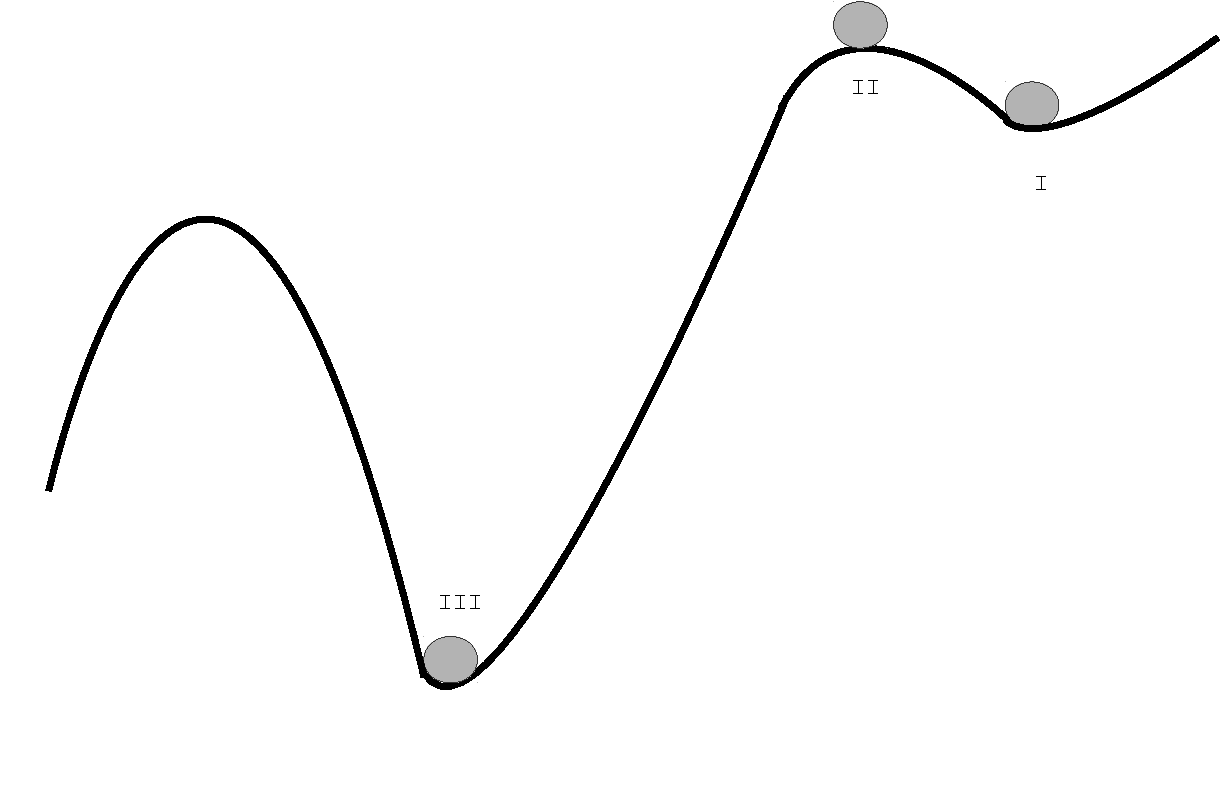
\includegraphics[width=0.4\columnwidth,clip]{./../Pics/Fig_SystemDefinition4}
        \caption{Potential energy variation in a particle motion.}\label{Chapter:Introduction:Fig:Domain4}
   \end{wrapfigure}

   Let's consider a particle initially at rest (state I in Fig.~\ref{Chapter:Introduction:Fig:Domain4}). The total energy associated with this particle is the sum of potential and kinetic energies (assuming that the particle is chemically inert and is kept at a constant temperature). If the particle is perturbed by a mechanical force of very small magnitude, it will eventually return to its initial state (\ie at a finite time), however if the perturbation is sufficiently large the particle is unlikely to return to the original state. In this scenario, the particle is said to be in a {\it unstable equilibrium}\index{Equilibrium!Mechanical!Unstable}. Now, let's assume that the particle is at state II, where any perturbation can move it to either state I or III. In such conditions, the particle is said to be in a {\it meta-stable equilibrium}\index{Equilibrium!Mechanical!Meta-stable}. Finally, if the particle is at state III, it will remain at this condition even under the influence of large perturbation. At such conditions, the particle is said to be in a {\it stable equilibrium}\index{Equilibrium!Mechanical!Stable}. If $E_{p}$ is the potential energy of the particle and $x$ is the displacement in the vertical direction, the equilibrium states can be described as
   \begin{equation}
      \begin{cases}
         \text{Stable equilibrium (III):}  & \frc{\partial E_{p}}{\partial x} = 0 \text{ and } \frc{\partial^{2} E_{p}}{\partial x^{2}} > 0; \\
          \\
         \text{Unstable equilibrium (II):}  & \frc{\partial E_{p}}{\partial x} = 0 \text{ and } \frc{\partial^{2} E_{p}}{\partial x^{2}} < 0; \\
          \\
         \text{Meta-stable equilibrium (I):}  & \frc{\partial E_{p}}{\partial x} = 0 \text{ and } \frc{\partial^{2} E_{p}}{\partial x^{2}} = 0; \\
      \end{cases}
   \end{equation}
   These mechanical equilibrium states can be extended to thermodynamic systems during phase changes, where the potential energy and the spatial coordinate are replaced by the {\it Gibbs free energy} and intensive/extensive properties, respectively.

   \bigskip

   The concept of thermal equilibrium is intuitively simple: if two or more bodies at distinct temperatures are in physical contact, the bodies will tend to a single temperature at a finite time. This principle is called the {\bf Zeroth Law} of thermodynamics and was first stated by J. C. Maxwell in 1872:
   \begin{MyBlock}{{\bf Zeroth Law of Thermodynamics (Maxwell, 1872) } }
     ``Bodies whose temperatures are equal to that of the same body have themselves equal temperatures.”
   \end{MyBlock}
   This definition enables the use of thermometers as devices to measure the temperature of bodies. Traditional thermometers have two components, a bulb containing mercury and a linear temperature scale. The mercury bulb is maintained at a relatively low temperature $\left(\text{\ie } T_{\text{th}}\le 35^{\circ}\text{C}\right)$, whereas a body is at temperature $T>T_{\text{th}}$. When the thermometer and the body are in contact, from the {\it zeroth law}, both will reach the same temperature $T$ at a finite time. The temperature difference triggers a volumetric expansion of the mercury that can be readily observed in the scaled glass column.

\clearpage   
\begin{FinalSummaryBlock}{Summary}
    In this chapter, some fundamental concepts of thermodynamic properties were revised and the their relationships with energy were introduced, also:
    \begin{itemize}
       \item Thermodynamics is the study of the transformations of energy;
       \item Energy can be defined as the capacity to produce work;
       \item Work is the transfer of energy by motion against an opposing force (Eqns.~\ref{Chpt01_Work1}-\ref{Chpt01_Work2};
       \item Heat is the transfer of energy  as a result of a temperature difference between the system and the surroundings;
       \item Definitions of system, surroundings and boundaries were stated in Section~\ref{Chapter:Introduction:Section:Introduction:SystemSurroundingsBoundaries};
       \item In open systems, mass and energy are allowed to freely flow across the boundaries of the system, whereas in closed system only energy is able to cross the borders at constant mass. In isolated (or adiabatic) system, neither energy nor mass can be trabsported across the borders;
       \item A state function is a property that depends only on the current state of the system and is independent of the origin of the state; 
       \item Thermal equilibrium is a condition in which no change of state occurs when two (or more) bodies are in contact with each other;
       \item Mechanical equilibrium is the condition of equality of pressure across the boundary of the system;
       \item The Zeroth Law of thermodynamics states that if a body {\it A} is in thermal equilibrium with a body {\it B}, and {\it B} is in thermal equilibrium with {\it C}, then {\it C} and {\it A} are also in thermal equilibrium;
    \end{itemize} 
   
     Most of these fundamentals concepts are familiar to you through other engineering courses. However, the remaining of this document strongly relies on this concepts and ideas, and you should understand all these concepts before moving forward.
\end{FinalSummaryBlock}

%\begin{MyTutorial}{\begin{center}{\bf Tutorial}\end{center}}
%  \begin{problem}
%  \end{problem}
%\end{MyTutorial}
